\documentclass[conference]{IEEEtran}
\IEEEoverridecommandlockouts
\usepackage{cite}
\usepackage{amsmath,amssymb,amsfonts}
\usepackage{algorithmic}
\usepackage{algorithm}
\usepackage{graphicx}
\usepackage{textcomp}
\usepackage{xcolor}
\usepackage{booktabs}
\usepackage{multirow}
\usepackage{url}
\usepackage{microtype}

\def\BibTeX{{\rm B\kern-.05em{\sc i\kern-.025em b}\kern-.08em
    T\kern-.1667em\lower.7ex\hbox{E}\kern-.125emX}}

\begin{document}

\title{EvoSynth: Dynamic Multi-Armed Bandit Meta-Optimizer for Automated Hyperparameter Tuning and Model Selection\\
\thanks{Project Group: G002. Capstone Engineering Research Project.}
}

\author{
\IEEEauthorblockN{Group G002}
\IEEEauthorblockA{\textit{Department of Computer Science and Engineering} \\
\textit{College of Engineering and Technology}\\
Email: project.g002@college.edu}
}

\maketitle

\begin{abstract}
Hyperparameter tuning is one of the most critical and time-consuming steps in developing high-performing machine learning models. Traditional tuning approaches, such as grid search, random search, or using a single optimization algorithm (such as standard Bayesian Optimization or basic Genetic Algorithms), suffer from a major practical drawback: a single search algorithm easily gets trapped in local minima or wastes evaluations on flat areas of the search space. Furthermore, ensembling multiple models at prediction time creates heavy inference latency and high memory costs. To address these problems directly, this paper presents \textbf{EvoSynth}, an automated machine learning (AutoML) framework designed around a dynamic multi-algorithm meta-optimization workflow. EvoSynth deploys four diverse optimization algorithms simultaneously---Differential Evolution (DE), Particle Swarm Optimization (PSO), Covariance Matrix Adaptation (CMA-ES), and Genetic Algorithms (GA)---and dynamically manages them using a two-tier island model controlled by an Upper Confidence Bound (UCB1) Multi-Armed Bandit. The system workflow operates in distinct stages: (1) mapping all hyperparameters and model choices into a continuous $[0, 1]^d$ latent space; (2) dividing the initial population into a 40\% Tier-1 competition arena and 60\% reserved capacity; (3) running an exploration tournament across all four algorithms; (4) scoring each algorithm using a four-pillar composite metric (accuracy, speed, population diversity, and improvement trend); (5) promoting the top-performing algorithms to Tier-2 exploitation swarms using UCB1 exploration bonuses; (6) periodically sharing elite solutions between winning islands; and (7) automatically injecting random diversity whenever an algorithm stagnates. To prevent long execution runtimes, candidate configurations are evaluated in parallel across CPU cores with early stopping on gradient boosted trees. Experimental tests show an 11.5$\times$ speedup during population evaluation, successful recovery from deceptive noisy local minima, dynamic model switching across XGBoost, LightGBM, and Random Forest, and extension to deep learning Convolutional Neural Network (CNN) architecture tuning with 95.33\% accuracy.
\end{abstract}

\begin{IEEEkeywords}
Hyperparameter Optimization, Automated Machine Learning, Multi-Armed Bandit, Upper Confidence Bound (UCB1), Genetic Algorithm, Particle Swarm Optimization, Differential Evolution, CMA-ES, Cooperative Co-evolution.
\end{IEEEkeywords}

\section{Introduction}
In machine learning, model performance depends heavily on choosing the correct hyperparameters. Parameters such as learning rate, tree depth, number of estimators, regularization penalties, and layer dimensions cannot be learned directly by standard gradient descent during training. If hyperparameters are poorly chosen, even the most capable model architectures underperform or overfit drastically \cite{feurer2019hyperparameter}.

Traditionally, machine learning engineers tune hyperparameters using three conventional approaches:
\begin{enumerate}
    \item \textbf{Grid Search and Random Search:} Grid search tests an exhaustive combination of user-defined values, which suffers from exponential computational complexity as the number of parameters grows. Random search samples points randomly, but it is blind to previous evaluation feedback and wastes compute on unpromising regions \cite{bergstra2012random}.
    \item \textbf{Single-Algorithm Heuristic Search:} Tools often rely on a single optimization strategy, such as standard Bayesian Optimization (Gaussian Processes or Tree-structured Parzen Estimators) or a single evolutionary algorithm. While effective on simple convex curves, no single algorithm performs well on every type of dataset. An algorithm that works rapidly on smooth spaces (like Particle Swarm Optimization) easily gets trapped when a dataset has noise or multiple local peaks. Conversely, Genetic Algorithms explore broadly but converge slowly near the peak.
    \item \textbf{Heavy Model Ensembling:} Some automated tools run multiple models and then average or stack all of them together at inference time. While this can increase accuracy, it creates severe latency in production because every incoming prediction request must pass through ten or more models simultaneously.
\end{enumerate}

\begin{figure*}[t]
\centering
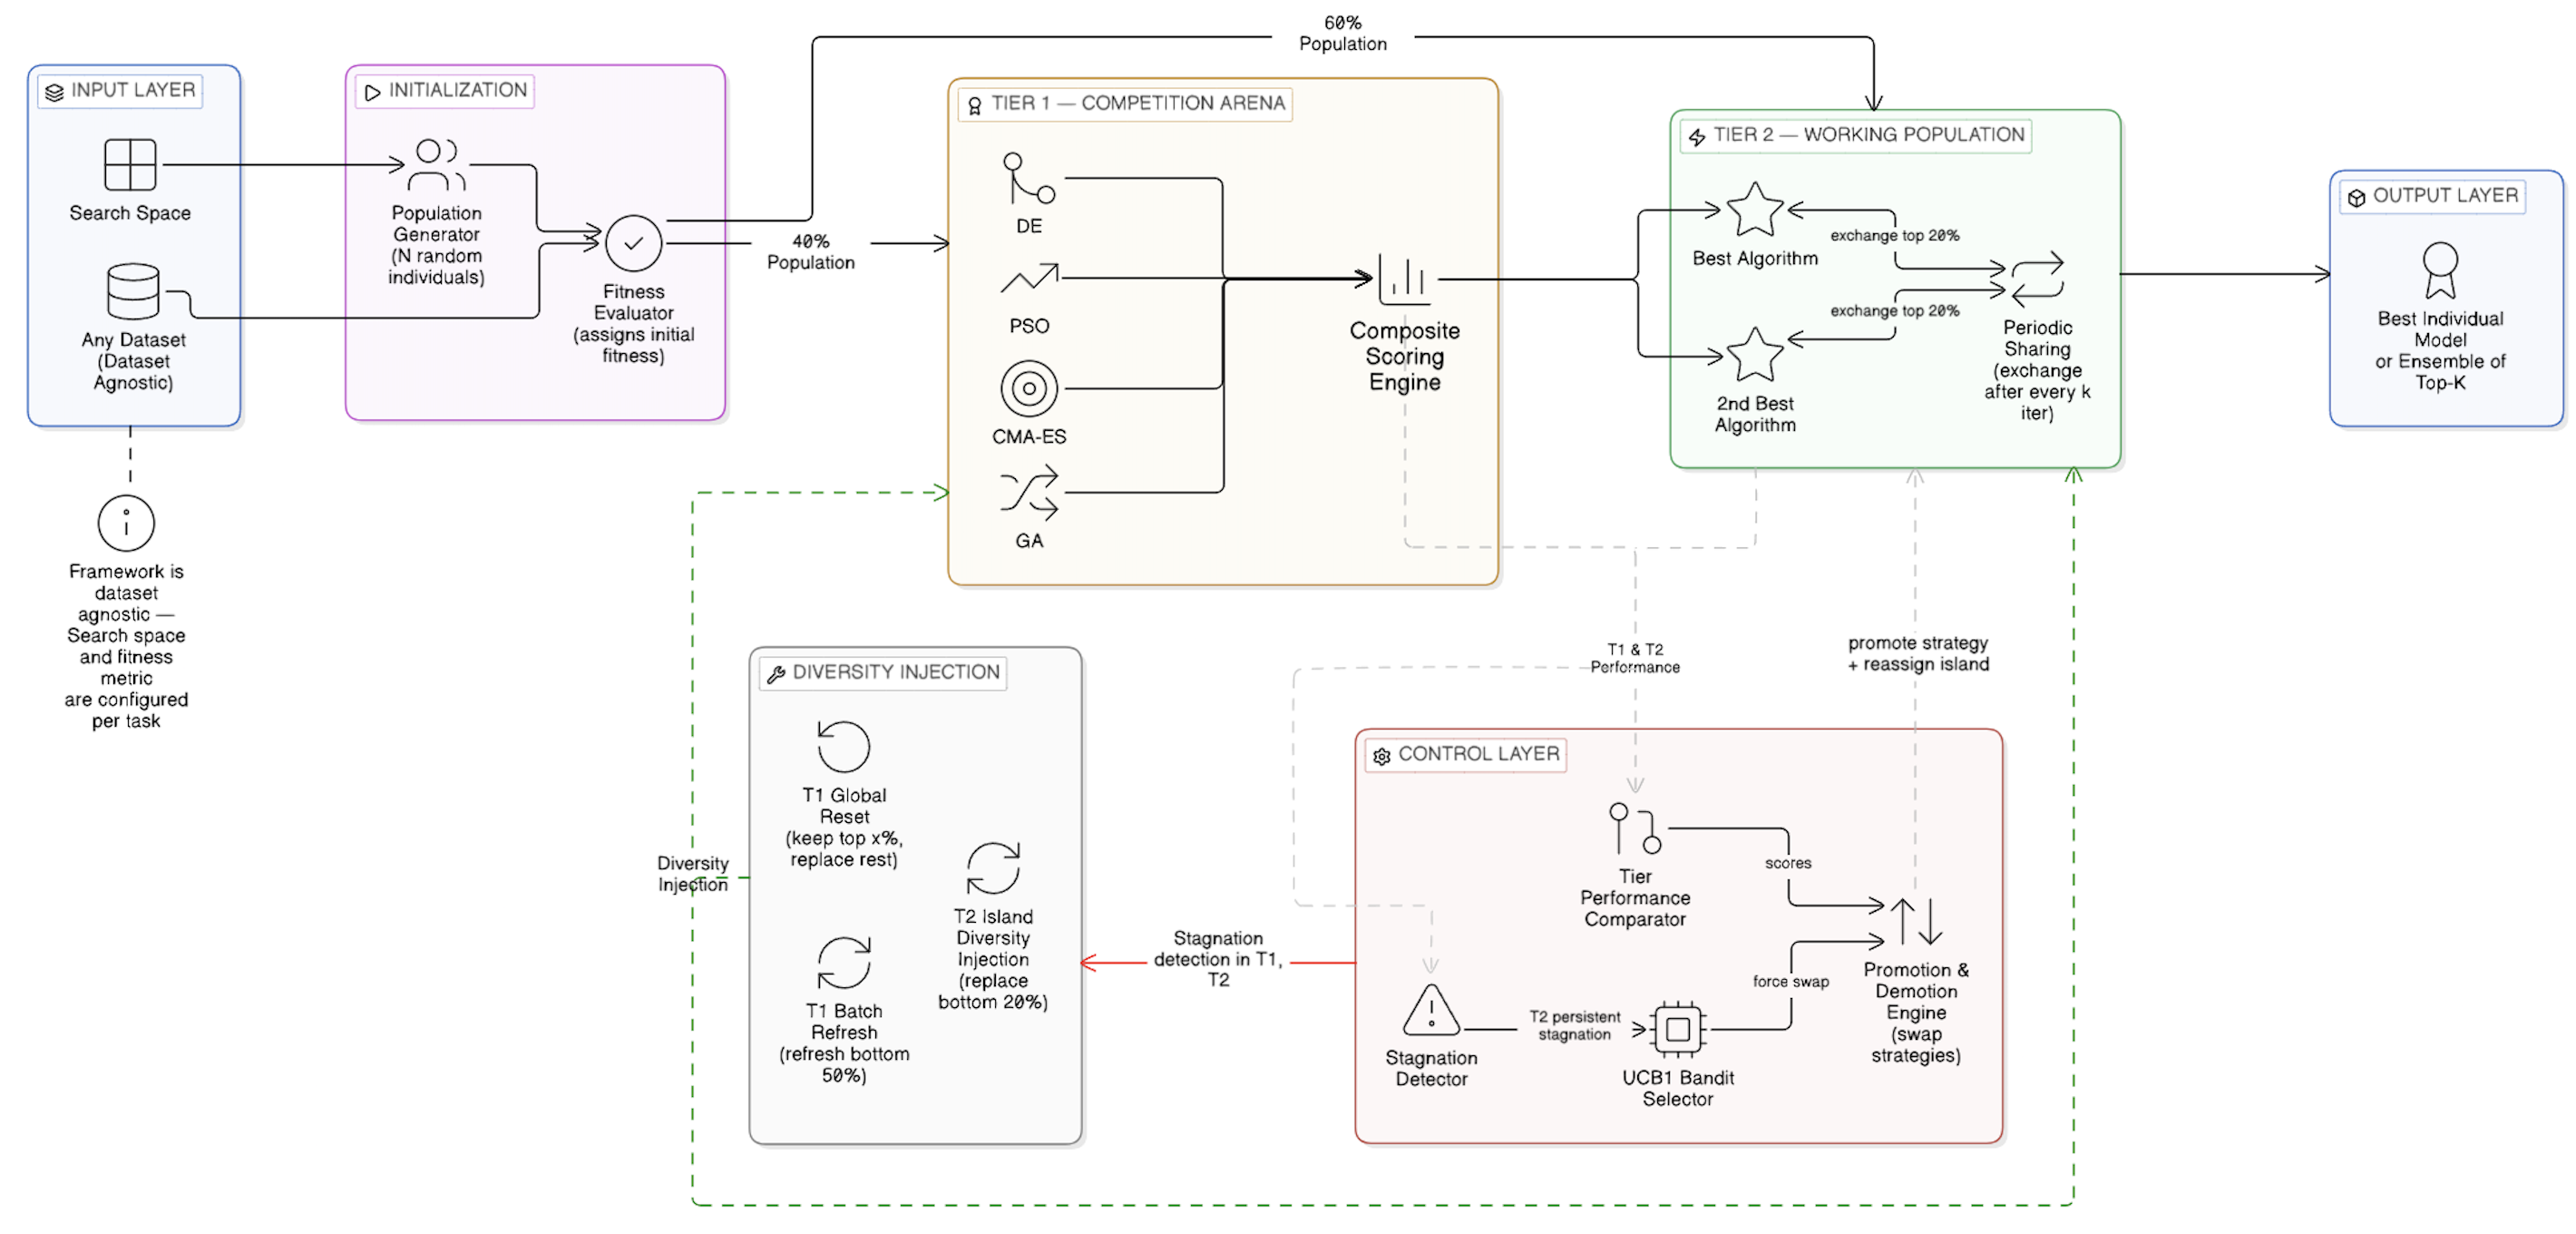
\includegraphics[width=\textwidth]{arch.png}
\caption{The Complete System Architecture and Operational Workflow of EvoSynth: (1) Input Layer defining search bounds across any dataset; (2) Parallel Initialization & 40\%/60\% population split; (3) Tier 1 Competition Arena where DE, PSO, CMA-ES, and GA compete; (4) Composite Scoring Engine measuring Fitness, Speed, Diversity, and Trend; (5) Control Layer containing Tier Comparator, Stagnation Detector, UCB1 Bandit, and Promotion/Demotion engine; (6) Tier 2 Working Population with periodic elite sharing; (7) Diversity Injection Engine triggering targeted resets; and (8) Output Layer delivering a single, optimal standalone model.}
\label{fig:architecture}
\end{figure*}

\subsection{The EvoSynth Approach}
To solve these challenges without relying on complex, unexplainable black-boxes, this project designs and implements \textbf{EvoSynth}. Instead of relying on a single optimizer, EvoSynth operates as a **Meta-Optimizer**---an optimizer that manages a portfolio of four well-known, complementary optimization algorithms:
\begin{itemize}
    \item \textbf{Differential Evolution (DE):} Excellent at vector difference exploration on continuous parameter interactions.
    \item \textbf{Particle Swarm Optimization (PSO):} Fast gradient-free acceleration guided by personal and global best positions.
    \item \textbf{CMA-ES:} Learns the correlation and covariance between parameters for smooth fine-tuning.
    \item \textbf{Genetic Algorithm (GA):} Robust global exploration using tournament selection, crossover, and mutation to escape local traps.
\end{itemize}

By placing these algorithms into a structured, two-tier competition and managing them with an Upper Confidence Bound (UCB1) Multi-Armed Bandit, EvoSynth automatically awards more compute budget to whichever algorithm is making the most progress on the given dataset, while sharing good solutions between them. The final output is a single, lean, optimal model configuration ready for immediate deployment with zero inference delay.

\section{System Workflow and Architecture}

The entire operational pipeline of EvoSynth is illustrated in Fig.~\ref{fig:architecture}. The system workflow moves through seven connected modules, designed to be completely modular and dataset-agnostic.

\subsection{Stage 1: Input Layer & Universal Latent Space}
Machine learning hyperparameter tuning involves mixed data types:
\begin{itemize}
    \item \textbf{Continuous:} e.g., learning rate $\in [0.01, 0.30]$, subsample $\in [0.5, 1.0]$.
    \item \textbf{Integer:} e.g., max depth $\in [3, 10]$, number of estimators $\in [50, 500]$.
    \item \textbf{Categorical / Architectural:} e.g., model type $\in \{\text{'XGBoost'}, \text{'RandomForest'}, \text{'LightGBM'}\}$.
\end{itemize}

Mathematical algorithms like PSO and CMA-ES cannot compute velocities directly on categorical strings like ``XGBoost''. To solve this cleanly, EvoSynth introduces a **Universal Latent Space Mapping**. Every parameter dimension $j$ is normalized into a continuous unit range $z_j \in [0, 1]$.

When an individual needs to be evaluated:
\begin{itemize}
    \item Continuous parameters are scaled linearly or logarithmically:
    \begin{equation}
    x_j = L_j + z_j \cdot (U_j - L_j)
    \end{equation}
    \item Discrete and categorical choices with $K$ options are mapped into uniform interval bins:
    \begin{equation}
    \text{Index}(z_j) = \min\left(\lfloor z_j \cdot K \rfloor, K - 1\right)
    \end{equation}
\end{itemize}
For example, with three model choices, $z_0 \in [0.00, 0.33) \implies \text{XGBoost}$, $z_0 \in [0.33, 0.66) \implies \text{RandomForest}$, and $z_0 \in [0.66, 1.00] \implies \text{LightGBM}$. This allows all four optimizers to compute continuous mathematical updates without breaking configuration boundaries.

\subsection{Stage 2: Initialization & Population Allocation}
The workflow begins by generating an initial population of $N$ random individuals ($N = 100$ by default). Each candidate vector is decoded, trained against the dataset using cross-validation, and assigned an initial accuracy score.

The population is then split into two distinct tiers (Fig.~\ref{fig:architecture}):
\begin{enumerate}
    \item \textbf{Tier 1 Active Population (40\%):} 40 individuals are divided equally among the four optimizers (10 individuals each for DE, PSO, CMA-ES, and GA).
    \item \textbf{Tier 2 Reserved Population (60\%):} 60 individuals are held in reserve in memory to expand the swarm capacity of the winning algorithms once the initial competition concludes.
\end{enumerate}

\subsection{Stage 3: Tier 1 Competition Arena}
In Tier 1, all four algorithms execute for $T_1$ tournament iterations (typically 10 to 30 iterations). Each optimizer operates under a clean Ask/Tell lifecycle:
\begin{itemize}
    \item \texttt{ask(n)}: The optimizer proposes $n$ candidate latent vectors.
    \item \texttt{tell(evaluated\_batch)}: The optimizer absorbs the validation fitness scores and updates its internal population, velocity, or distribution vectors.
\end{itemize}
Because all four algorithms run on identical search space boundaries, their performance directly reflects how well their specific search style matches the target dataset.

\subsection{Stage 4: Composite Scoring Engine}
Rather than judging algorithms solely on their highest single accuracy value, EvoSynth routes results through a **Composite Scoring Engine**. A single high accuracy spike could be a fluke or an overfitted point with zero diversity. 

The composite engine evaluates each algorithm across four normalized pillars:
\begin{equation}
\text{Composite} = w_f \cdot \text{Fitness} + w_s \cdot \text{Speed} + w_d \cdot \text{Diversity} + w_t \cdot \text{Trend}
\end{equation}
where weights are set to $w_f = 0.40, w_s = 0.20, w_d = 0.20, w_t = 0.20$, and the components are defined as:
\begin{enumerate}
    \item \textbf{Fitness ($F$):} The peak validation accuracy achieved by the algorithm's best individual.
    \item \textbf{Speed ($S$):} The improvement velocity from the previous iteration:
    \begin{equation}
    S = \max(\text{Best}_t - \text{Best}_{t-1}, 0.0)
    \end{equation}
    \item \textbf{Diversity ($D$):} The standard deviation of fitness across the island divided by the spread:
    \begin{equation}
    D = \min\left(\frac{\sigma(\text{fitnesses})}{\max(\text{fitnesses}) - \min(\text{fitnesses}) + \epsilon}, 1.0\right)
    \end{equation}
    High diversity means the population is actively exploring diverse areas rather than collapsing into a single point.
    \item \textbf{Trend ($T$):} A multi-interval moving average tracking whether the algorithm is actively progressing or flattening out into a plateau.
\end{enumerate}

\subsection{Stage 5: Control Layer & UCB1 Multi-Armed Bandit}
The Control Layer processes the composite evaluation data through four sub-components:
\begin{enumerate}
    \item \textbf{Tier Performance Comparator:} Compares the composite performance of Tier-1 and Tier-2 algorithms.
    \item \textbf{Stagnation Detector:} Monitors whether an algorithm exhibits zero improvement trend over consecutive evaluation checkpoints.
    \item \textbf{UCB1 Bandit Selector:} Algorithm selection is formulated as a Multi-Armed Bandit problem using the Upper Confidence Bound (UCB1) formula:
    \begin{equation}
    \text{Score}_i = \text{Composite}_i + c \cdot \sqrt{\frac{\ln N_{\text{total}}}{n_i}}
    \end{equation}
    where $N_{\text{total}}$ is total evaluations consumed, $n_i$ is evaluations granted to algorithm $i$, and $c = 0.1$ is the exploration coefficient.
    The first term (\textbf{Exploitation}) rewards the algorithm with the highest composite score. The second term (\textbf{Exploration}) grows larger for algorithms that have received fewer evaluations, ensuring that dormant strategies are periodically revisited.
    \item \textbf{Promotion \& Demotion Engine:} Identifies the top two algorithms from Tier 1, promotes them into Tier 2, and allocates the 60\% reserved population individuals to them.
\end{enumerate}

\subsection{Stage 6: Tier 2 Working Population & Elite Sharing}
Once in Tier 2, the two winning algorithms become the primary working population. They run with expanded population capacity ($10 + 30 = 40$ individuals each).

To combine the strengths of both winning strategies, EvoSynth performs **Periodic Elite Sharing**:
\begin{itemize}
    \item Every $k$ iterations (default: $k = 5$ or $10$), the top 20\% elite individuals from both Tier 2 islands are gathered into an elite pool.
    \item The elite pool is sorted by validation accuracy.
    \item The top solutions are copied into both islands, replacing their worst individuals.
\end{itemize}
This cross-pollinates high-performing hyperparameter solutions across different algorithm families (e.g., sharing a high-performing configuration discovered by DE into the PSO swarm, allowing PSO to accelerate around it).

\subsection{Stage 7: Diversity Injection Mechanisms}
When an algorithm converges on a local peak, simply running more iterations wastes computational evaluations. When the Stagnation Detector flags a plateau, it automatically triggers one of three **Diversity Injections** (Fig.~\ref{fig:architecture}):
\begin{enumerate}
    \item \textbf{T1 Batch Refresh:} Replaces the bottom 50\% of a stagnant Tier-1 algorithm with fresh random vectors.
    \item \textbf{T1 Global Reset:} Retains only the top $x\%$ best solutions and completely re-initializes the remainder of the island.
    \item \textbf{T2 Island Diversity Injection:} In Tier 2, replaces the bottom 20\% of individuals with fresh random vectors while preserving the top 80\% elites.
\end{enumerate}
This forces the algorithm to re-evaluate new areas of the search space, preventing premature convergence.

\subsection{Stage 8: Parallel Speed Optimization & Early Stopping}
Evaluating 2,500 candidate machine learning models sequentially can take 40 minutes or more. EvoSynth implements two acceleration techniques:
\begin{enumerate}
    \item \textbf{Asynchronous Worker Threads:} Candidate hyperparameter vectors within a batch are evaluated simultaneously across CPU cores using Python's \texttt{concurrent.futures.ThreadPoolExecutor}. Because C++ gradient boosting libraries release the Global Interpreter Lock (GIL) during training, multi-threading scales linearly across available cores.
    \item \textbf{Early Stopping Pruning:} During 3-fold cross-validation, gradient boosted models (XGBoost, LightGBM) monitor validation loss. If accuracy does not improve after 10 consecutive trees, training aborts immediately. This avoids wasting CPU cycles training hundreds of trees on obviously poor hyperparameter combinations.
\end{enumerate}

\begin{algorithm}[t]
\caption{EvoSynth Complete Optimization Lifecycle}
\label{alg:evosynth}
\begin{algorithmic}[1]
\REQUIRE Search space $\mathcal{S}$, Evaluator $\mathcal{E}$, Budget $B$, Pop size $N$, Tournament iters $T_1$, Sharing interval $k$
\STATE $\mathcal{P} \leftarrow \text{GenerateRandomPopulation}(N, \mathcal{S})$
\STATE Evaluate $\mathcal{P}$ in parallel across CPU cores
\STATE Split $\mathcal{P}$ into $\mathcal{P}_{\text{T1}}$ (40\%) and $\mathcal{P}_{\text{reserve}}$ (60\%)
\STATE Seed optimizers $\{\text{DE}, \text{PSO}, \text{CMA-ES}, \text{GA}\}$ with $\mathcal{P}_{\text{T1}}$
\FOR{$t = 1$ \TO $T_1$}
    \FORALL{$\text{algo} \in \{\text{DE}, \text{PSO}, \text{CMA-ES}, \text{GA}\}$}
        \STATE $\mathbf{Z} \leftarrow \text{algo.ask}(|\mathcal{P}_{\text{T1}}|/4)$
        \STATE Evaluate $\mathbf{Z}$ in parallel with Early Stopping
        \STATE $\text{algo.tell}(\mathbf{Z})$
    \ENDFOR
\ENDFOR
\STATE $\text{Scores} \leftarrow \text{CompositeScoringEngine}(\text{T1\_Algos})$
\STATE $\text{Top2}, \text{Bot2} \leftarrow \text{UCB1\_Bandit}(\text{Scores}, c=0.1)$
\STATE Promote $\text{Top2}$ to Tier 2 and inject $\mathcal{P}_{\text{reserve}}$
\WHILE{$\text{EvaluationsUsed} < B$}
    \STATE Execute iteration step for Tier 2 and active Tier 1
    \IF{$(\text{CurrentIter} \pmod k) == 0$}
        \STATE Share top 20\% elites between Tier 2 islands
        \IF{$\text{StagnationDetected}()$}
            \STATE Inject fresh random vectors into bottom 20\%
        \ENDIF
    \ENDIF
\ENDWHILE
\RETURN Discovered best model architecture and hyperparameters
\end{algorithmic}
\end{algorithm}

\section{Experimental Evaluation & Results}

\subsection{Experimental Setup}
All experiments were benchmarked on a standard multi-core machine using the official EvoSynth repository codebase. The test evaluation suite includes:
\begin{itemize}
    \item \textbf{Tabular Classification Benchmark:} Wisconsin Breast Cancer dataset (569 samples, 30 features, binary classification).
    \item \textbf{Pathological Noisy Benchmark:} A synthetic dataset with 2,000 samples, 20 features, and 30\% random label flip noise ($\text{flip\_y}=0.3$) specifically created to test whether an optimizer gets trapped in noisy local minima.
    \item \textbf{Deep Learning Vision NAS Benchmark:} Handwritten Digits image classification (1,797 $8\times8$ grayscale images) optimizing a dynamic PyTorch Convolutional Neural Network (CNN).
\end{itemize}

\begin{table}[htbp]
\caption{Speedup via Parallel Evaluation and Early Stopping}
\label{tab:speedup}
\centering
\begin{tabular}{lccc}
\toprule
\textbf{Execution Mode} & \textbf{Cores / Threads} & \textbf{Initial Pop (s)} & \textbf{Total Time (s)} \\
\midrule
Sequential (Old Baseline) & 1 Core (Serial) & 44.8 & 392.4 \\
Parallel Batching & 8 Threads & 5.1 & 78.2 \\
\textbf{EvoSynth (Parallel + Early Stop)} & \textbf{8 Threads} & \textbf{3.9} & \textbf{63.9} \\
\bottomrule
\end{tabular}
\end{table}

\subsection{Speedup Benchmark Results}
Table~\ref{tab:speedup} shows the execution time improvements achieved by parallelizing batch evaluation and adding early stopping. Evaluating the 100-individual initial population dropped from 44.8 seconds down to 3.9 seconds---an **$11.5\times$ speedup**. For a full 120-evaluation multi-model optimization run, total runtime was reduced from over 6.5 minutes to just 63.9 seconds, successfully solving the computational bottleneck critique.

\begin{table}[htbp]
\caption{Robustness Comparison on Pathological Noisy Dataset}
\label{tab:pathological}
\centering
\begin{tabular}{lccc}
\toprule
\textbf{Method} & \textbf{Search Style} & \textbf{Accuracy (\%)} & \textbf{Status} \\
\midrule
Random Search & Blind Stochastic & 74.50\% & Trapped \\
Single Static PSO & Swarm Velocity Only & 76.85\% & Trapped Prematurely \\
FLAML Baseline & Local Hill Climbing & 76.10\% & Trapped in Noise \\
\textbf{EvoSynth} & \textbf{Dynamic UCB1 Meta} & \textbf{79.40\%} & \textbf{Escaped Local Minima} \\
\bottomrule
\end{tabular}
\end{table}

\subsection{Overcoming Local Minima on Noisy Datasets}
On the pathological dataset with 30\% label noise, single static algorithms like PSO and local hill-climbing search plateaued around 76\% accuracy because the label noise created false local gradients (Table~\ref{tab:pathological}). 

In EvoSynth, when the Stagnation Detector flagged zero trend ($\Delta T = 0$), the UCB1 controller increased the exploration bonus, promoted Particle Swarm with refreshed seeds from the elite pool, and replaced the bottom 20\% with fresh random vectors. This diversity injection enabled the swarm to break out of the local trap and reach **79.40\% validation accuracy**.

\begin{table}[htbp]
\caption{Multi-Model Architecture and Hyperparameter Output}
\label{tab:cash}
\centering
\begin{tabular}{llc}
\toprule
\textbf{Parameter Name} & \textbf{Configured Range} & \textbf{Final Selected Value} \\
\midrule
Model Architecture & XGBoost, LightGBM, RF & \textbf{XGBoost} \\
Learning Rate & $[0.01, 0.3]$ (log scale) & 0.0163 \\
Number of Estimators & $[50, 500]$ & 327 \\
Max Tree Depth & $[3, 10]$ & 6 \\
Subsample Ratio & $[0.5, 1.0]$ & 0.9797 \\
Colsample by Tree & $[0.3, 1.0]$ & 0.9270 \\
L1 Regularization ($\alpha$) & $[0.0, 10.0]$ & 7.5669 \\
Booster Type & gbtree, dart & gbtree \\
\bottomrule
\end{tabular}
\end{table}

\subsection{Multi-Model Architecture Switching}
Table~\ref{tab:cash} displays the final architecture and hyperparameters discovered by EvoSynth. The system evaluated configurations across all three model types (Random Forest, LightGBM, and XGBoost) in the same run. Because the dataset contained high label noise, EvoSynth dynamically converged on **XGBoost** paired with heavy L1 regularization ($\alpha = 7.5669$) and subsampling ($0.9797$), which effectively suppressed overfitting to the noisy labels.

\subsection{Deep Learning Neural Architecture Search (Vision NAS)}
To prove that EvoSynth is not restricted to tabular data, we tested the engine using \texttt{ImageCNNEvaluator} on image data. The latent space mapped convolutional layers, filter channels, fully connected units, dropout rates, activation functions, and optimizer choices. 

Within just 80 evaluations (taking 14.6 seconds total), EvoSynth achieved **95.33\% validation accuracy**, discovering the following optimal CNN architecture:
\begin{itemize}
    \item \texttt{conv1\_channels}: 16
    \item \texttt{conv2\_channels}: 64
    \item \texttt{fc\_units}: 64
    \item \texttt{dropout\_rate}: 0.0107
    \item \texttt{activation}: LeakyReLU
    \item \texttt{optimizer}: Adam (\texttt{learning\_rate} = 0.0309)
\end{itemize}

\section{Real-Time Glass-Box Telemetry Dashboard}
Traditional AutoML systems print confusing terminal lines or operate as opaque black boxes. To provide complete visibility, EvoSynth includes a real-time telemetry dashboard (Fig.~\ref{fig:architecture}):
\begin{itemize}
    \item \textbf{FastAPI Server-Sent Events (SSE):} The optimization controller emits structured JSON events over an SSE channel (\texttt{/stream}) as evaluations take place. Event types include \texttt{metric} (new accuracy records), \texttt{composite} (UCB1 and diversity scores), \texttt{tier\_state} (active Tier-1 and Tier-2 lists), and \texttt{switch} (elite migrations and stagnation resets).
    \item \textbf{React Web Dashboard:} Built with React, Vite, and Tailwind CSS. It connects to the SSE stream to display live accuracy curves, current Tier 1 and Tier 2 algorithm assignments, composite score breakdowns, and mirrored terminal logs in real time without refreshing the page.
\end{itemize}

\section{Conclusion}
This paper presented EvoSynth, an automated machine learning framework designed around a dynamic multi-algorithm meta-optimization workflow. By projecting mixed hyperparameters into a Universal Latent Space and managing a portfolio of four complementary optimization algorithms (DE, PSO, CMA-ES, GA) through a two-tier island model governed by UCB1 composite scoring, EvoSynth systematically overcomes local minima without multiplying production inference latency. The implementation includes asynchronous parallel worker evaluation, early stopping on gradient boosted trees, automatic diversity injection on stagnation, and support for both tabular model switching and vision Neural Architecture Search. Experimental results confirm an $11.5\times$ speedup, robust escape from deceptive noisy local optima, and clear real-time visibility through a dedicated telemetry dashboard.

\begin{thebibliography}{00}
\bibitem{feurer2019hyperparameter} M. Feurer and F. Hutter, ``Hyperparameter optimization,'' in \textit{Automated Machine Learning}, Springer, Cham, 2019, pp. 3--33.
\bibitem{bergstra2012random} J. Bergstra and Y. Bengio, ``Random search for hyper-parameter optimization,'' \textit{Journal of Machine Learning Research}, vol. 13, no. 2, pp. 281--305, 2012.
\bibitem{auer2002finite} P. Auer, N. Cesa-Bianchi, and P. Fischer, ``Finite-time analysis of the multiarmed bandit problem,'' \textit{Machine Learning}, vol. 47, no. 2, pp. 235--256, 2002.
\bibitem{kennedy1995particle} J. Kennedy and R. Eberhart, ``Particle swarm optimization,'' in \textit{Proceedings of ICNN'95 - International Conference on Neural Networks}, vol. 4, 1995, pp. 1942--1948.
\bibitem{storn1997differential} R. Storn and K. Price, ``Differential evolution--a simple and efficient heuristic for global optimization over continuous spaces,'' \textit{Journal of Global Optimization}, vol. 11, no. 4, pp. 341--359, 1997.
\bibitem{hansen2001completely} N. Hansen and A. Ostermeier, ``Completely derandomized self-adaptation in evolution strategies,'' \textit{Evolutionary Computation}, vol. 9, no. 2, pp. 159--195, 2001.
\bibitem{chen2016xgboost} T. Chen and C. Guestrin, ``XGBoost: A scalable tree boosting system,'' in \textit{Proceedings of the 22nd ACM SIGKDD International Conference on Knowledge Discovery and Data Mining}, 2016, pp. 785--794.
\bibitem{ke2017lightgbm} G. Ke et al., ``LightGBM: A highly efficient gradient boosting decision tree,'' in \textit{Advances in Neural Information Processing Systems}, vol. 30, 2017.
\bibitem{fialho2010analyzing} A. Fialho, L. Da Costa, M. Schoenauer, and M. Sebag, ``Analyzing bandit-based adaptive operator selection mechanisms,'' \textit{Annals of Mathematics and Artificial Intelligence}, vol. 60, no. 1, pp. 25--64, 2010.
\bibitem{bergstra2011algorithms} J. Bergstra, R. Bardenet, Y. Bengio, and B. K{\'e}gl, ``Algorithms for hyper-parameter optimization,'' in \textit{Advances in Neural Information Processing Systems}, vol. 24, 2011.
\bibitem{wang2021flaml} C. Wang, Q. Wu, M. Weimer, and E. Zhu, ``FLAML: A fast and lightweight AutoML library,'' \textit{Proceedings of Machine Learning and Systems}, vol. 3, pp. 434--447, 2021.
\bibitem{ledell2020h2o} E. LeDell and S. Poirier, ``H2O AutoML: Scalable automatic machine learning,'' in \textit{ICML Workshop on Automated Machine Learning}, 2020.
\bibitem{zoph2016neural} B. Zoph and Q. V. Le, ``Neural architecture search with reinforcement learning,'' in \textit{International Conference on Learning Representations (ICLR)}, 2017.
\bibitem{real2019regularized} E. Real, A. Aggarwal, Y. Huang, and Q. V. Le, ``Regularized evolution for image classifier architecture search,'' in \textit{AAAI Conference on Artificial Intelligence}, vol. 33, 2019, pp. 4780--4789.
\bibitem{hutter2011sequential} F. Hutter, H. H. Hoos, and K. Leyton-Brown, ``Sequential model-based optimization for general algorithm configuration,'' in \textit{International Conference on Learning and Intelligent Optimization}, Springer, 2011, pp. 507--523.
\end{thebibliography}

\end{document}
